% !TeX root = ../main.tex

\chapter{石墨烯结构}

\section{石墨的结构}
石墨为层状结构(图~\ref{fig:graphiteStructure}),每一层中的6个碳原子构成平面网状结构,层和层之间以范德瓦尔斯力连接。

天然石墨一般有三种存在形式:无定形态、高结晶态、天然鳞片状。鳞片状石墨纯度较高,可达99\%,因更具有方向性,它比其它形式的石墨存在更大的研究价值和使用价值。

从C原子的堆积方式来看,石墨的C原子堆积方式主要有两种:一是以ABAB的顺序重复,具有六方晶系对称性,称为六方石墨;另一种结构是以ABCABC的顺序重复堆积,具有三方晶系对称性,称为三方石墨。六方石墨和三方石墨层间距离都为$0.335nm$,层间作用力为范德华力。

{\begin{figure}
    \centering
    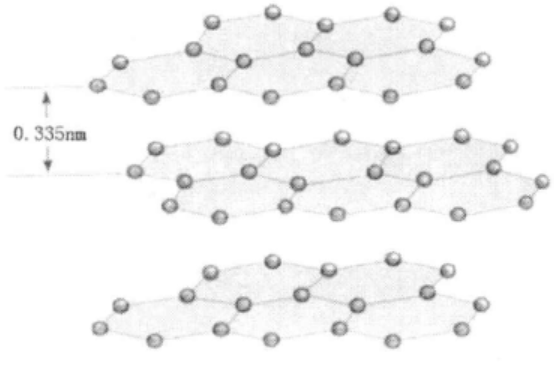
\includegraphics[scale=0.6]{img/石墨的结构图.png}
    \caption{石墨的结构图}
    \label{fig:graphiteStructure}
\end{figure}}

\section{石墨烯的结构}
石墨烯是各种石墨结构的母体,是构建其它维数碳质材料的基本单元。二维石墨烯多层叠加形成三维的石墨体,卷曲形成一维结构的碳纳米管,包裹形成零维的球形富勒烯(图\ref{fig:grapheneStructure})。所以这种最基础的结构是构筑其它材料的原型。

\begin{figure}
    \centering
    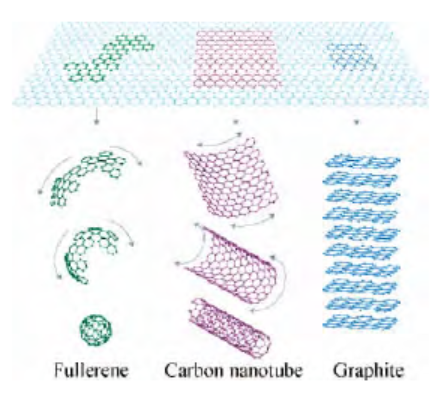
\includegraphics{img/石墨烯和几种炭材料的结构.png}
    \caption{石墨烯和几种炭材料的结构}
    \label{fig:grapheneStructure}
\end{figure}

单层石墨烯的厚度约$0.35nm$,碳-碳键长为$0.142nm$,理论上理想的单层石 墨烯的比表面积达$2630m^{2}/g$。

石墨烯中碳原子呈六环结构排列,这样独特的稳定结构使石墨烯具有较高的拉伸弹性模量和抗拉强度、优良的导热性能、零带隙、电子-空穴迁移率高。当施加外部机械力时,碳原子层就会弯曲变形来适应外力,而不必使碳原子重新排列,这样就保持了结构的稳定。

石墨烯晶体结构中每个元胞包含两个碳原子,四个价电子的其中三个分别与邻近碳原子产生$sp^{2}$轨道杂化形成三个$\sigma$键,另外一个$p$轨道电子贡献给非局域化的$\pi$和$\pi^{*}$键,分别形成最高占据电子轨道和最低非占据电子轨道。而石墨烯的$\pi$和$\pi^{*}$键布里渊区K点处退化,费米面收缩成一个点,形成无带隙的金属能带结构(图~\ref{fig:grapheneElectrical})。

\begin{figure}
    \centering
    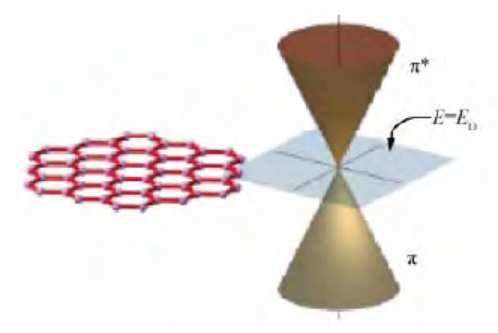
\includegraphics[scale=0.6]{img/单层石墨烯的电子结构.png}
    \caption{单层石墨烯的电子结构}
    \label{fig:grapheneElectrical}
\end{figure}